
\section{Metodologia}
	\subsection{Materiais}
%\begin{frame}{}
%	\centering \Huge \color{blue} \textbf{Metodologia} \\[1cm] Materiais
%\end{frame}
	\begin{frame}{Materiais}
		\begin{itemize}
			\item Itens utilizados para a realização da pesquisa:
			\bigskip
			\begin{enumerate}
  				\setlength\itemsep{1em}
				\item \textbf{Dispositivo Lógico Programável:}  FPGA;
%				\item Analisador Lógico Saleae Logic 16;
				\item \textbf{Plataforma de Prototipagem:}  Arduino;
				\item \textbf{Sistema Operacional:} GNU/Linux.
			\end{enumerate}
		\end{itemize}
	\end{frame}




	\subsection{Métodos}
	\begin{frame}{Método - \textit{Software}}
		\begin{multicols}{2}
				%\begin{itemize}
				%	\item Escrita do \textit{Driver}:
					\begin{itemize}
						\item Pesquisa no livro \textbf{Linux Driver Driver 3$^{\circ}$ Edição} disponível gratuitamente para leitura e impressão\footnote{\url{https://www.makelinux.net/ldd3/}.} \cite{corbet2005linux}.
						\item Utilizou-se de \textbf{\textit{mailing lists}} do sítio \url{linux-usb.org} para suprimir dúvidas.
						%https://www.kernel.org/doc/Documentation/driver-model/
						\item Documentação do Linux Kernel\footnote{\url{https://www.kernel.org/doc/Documentation/driver-model/}.}.
						\item Estudo de \textit{Drivers} do Kernels.
					\end{itemize}
				%\end{itemize}
			\columnbreak
				\begin{figure}[p]
					\centering
					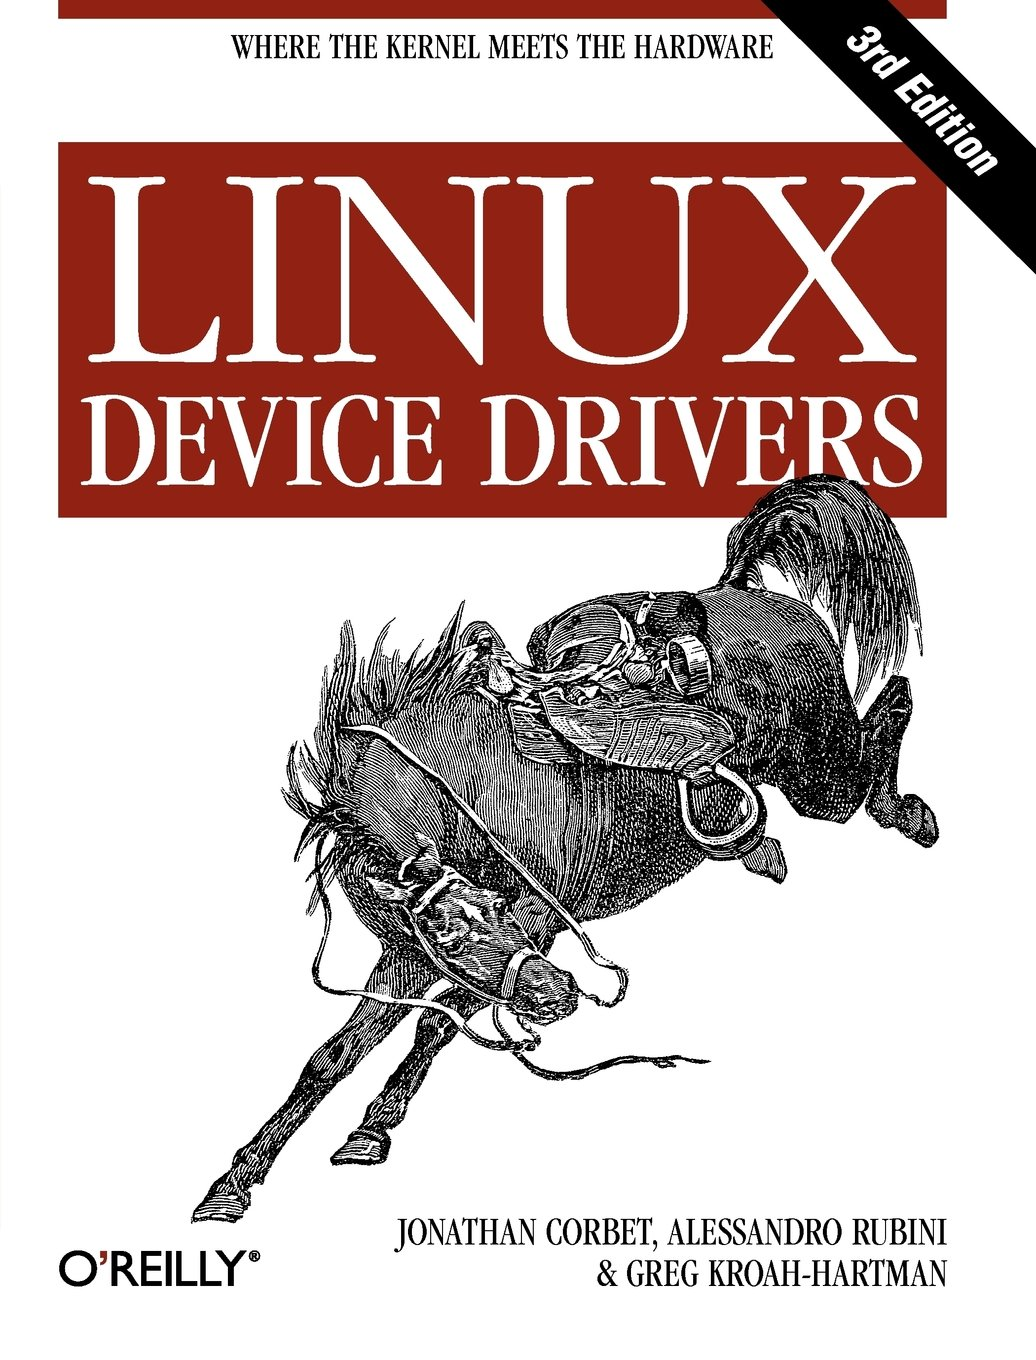
\includegraphics[width=0.33\textwidth]{img/livro.jpg}
					\caption{Linux Device Driver 3$^{\circ}$ Edição \cite{corbet2005linux}.}
					\label{fig:ldd3}
				\end{figure}
		\end{multicols}
	\end{frame}

	\begin{frame}{Método - \textit{Hardware}}
		\begin{itemize}
			\setlength\itemsep{2.2em}
			\item Cursos introdutório sobre \textbf{Linguagem VHDL e Sintetização de Projetos em Hardware}.
			%\item Em seguida, com a pesquisa aplicada, aprimorou-se o desenvolvimento de projetos de maior porte e mais complexos.
		\end{itemize}
	\end{frame}
	\begin{frame}{Método}
		\begin{enumerate}
			\setlength\itemsep{1.2em}
			%\begin{itemize}
				%\item A apredizagem e desenvolvimento foram iniciados em projeto de pesquisa aplicada\footnote{ANEXO VI - Edital no 156/2013, protocolo 23208.01490/2013DV.};
			%\end{itemize}
			\item Pesquisa sobre \textbf{desenvolvimento de \textit{Drivers}}:
			\begin{itemize}
				\item Características principais;
				\item Tipos;
				\item Escrita;
				\item Compilação.
			\end{itemize}
			\item FPGA:
			\begin{itemize}
				\item Escrever procedimentos de envio e recebimento de dados;
				\item Máquina de estado controladora.
			\end{itemize}
			\item \textbf{Interconectar} as duas extremidades usando o \textbf{Arduino}.
		\end{enumerate}
	\end{frame}
	\begin{frame}{Método - Estrutura do Projeto}
		\begin{figure}[p]
			\centering
			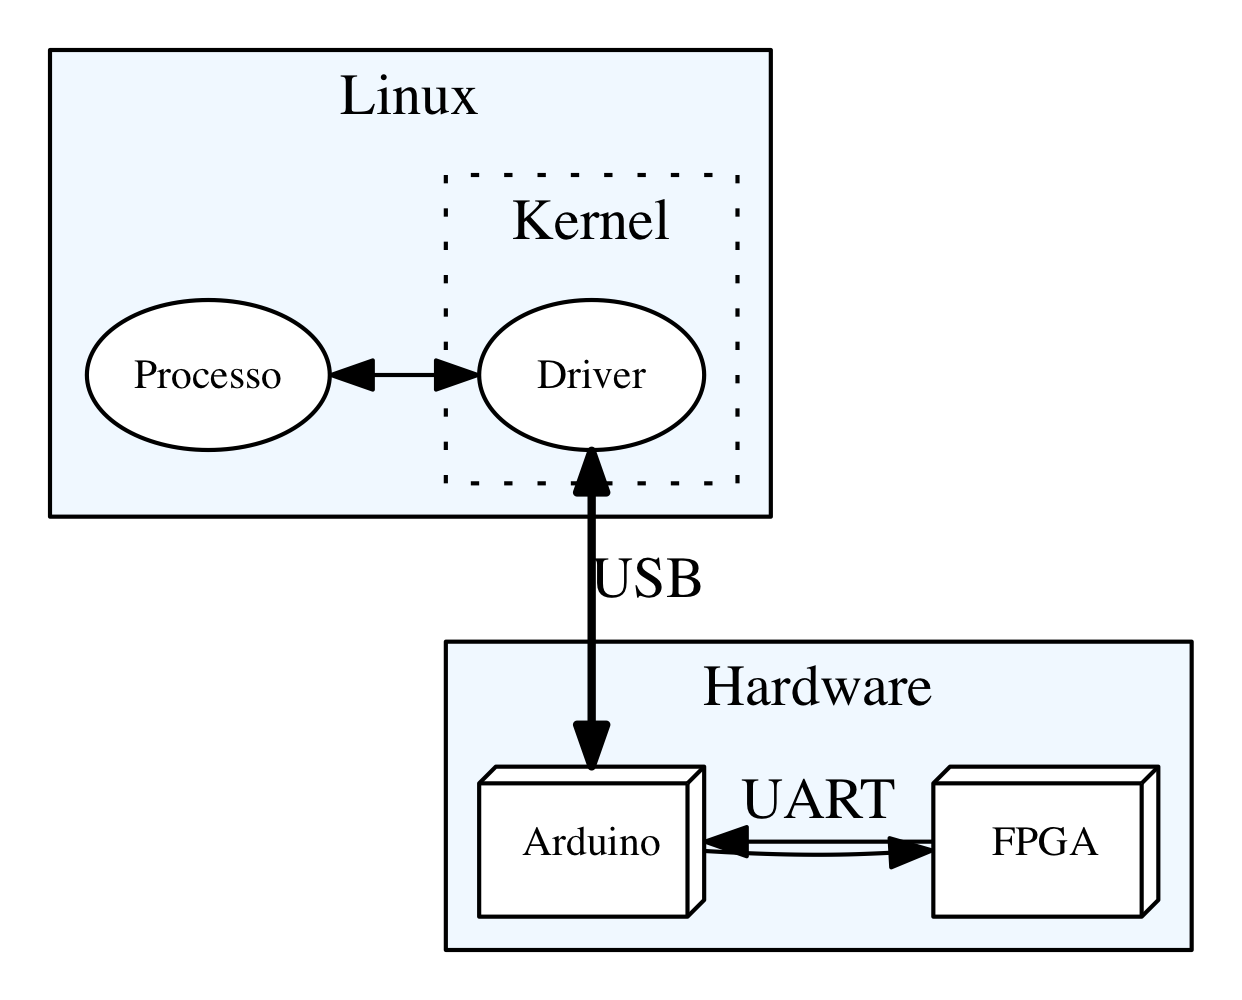
\includegraphics[width=0.72\textwidth]{img/projeto.png}
			\caption{Representação do projeto numa visão geral.}
			\label{fig:projeto}
		\end{figure}
	\end{frame}









